\documentclass[border=10pt]{standalone}
\usepackage{tikz}
\usetikzlibrary{shapes.geometric, positioning}

\tikzset{%
  db/.style = {cylinder, draw},
  tool/.style = {rectangle, draw},
  data/.style = {},
  func/.style = {},
  fake/.style = {}
}


\begin{document}
  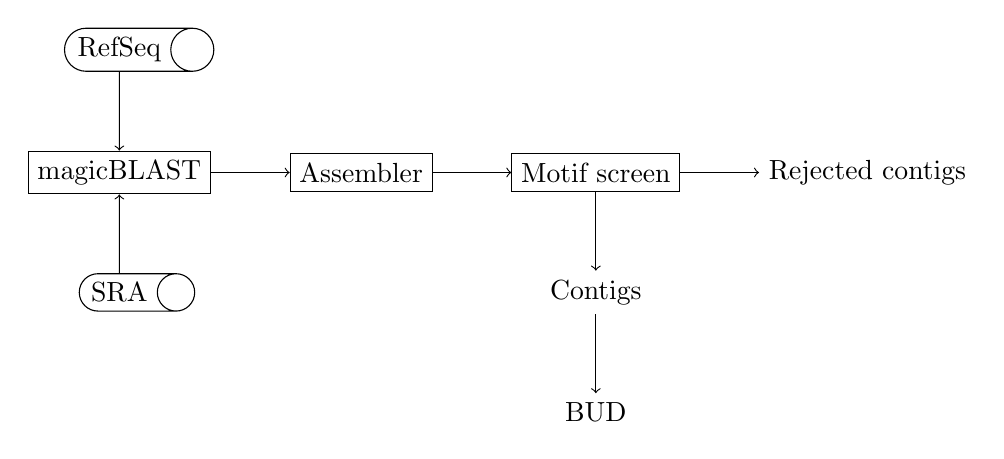
\begin{tikzpicture}
    \pgfdeclarelayer{background}
    \pgfdeclarelayer{foreground}
    \pgfsetlayers{background,main,foreground}

    \node (mapper)    [tool] {magicBLAST};
    \node (refseq)    [db,  above = of mapper] {RefSeq};
    \node (sra)       [db,  below = of mapper] {SRA};
    \node (asm)       [tool, right = of mapper]             {Assembler};
    \node (mscreen)   [tool, right = of asm]                {Motif screen};
    \node (reject)    [data, right = of mscreen]            {Rejected contigs};
    \node (ctgs)      [data, below = of mscreen]            {Contigs};
    \node (bud)       [func, below = of ctgs]               {BUD};

    \path[->] (refseq)    edge (mapper)
              (sra)       edge (mapper)
              (mapper)    edge (asm)
              (asm)       edge (mscreen)
              (mscreen)   edge (reject)
                          edge (ctgs)
              (ctgs)      edge (bud);
    %\begin{pgfonlayer}{background}
      %\path (mapper.west |- mapper.north)+(-0.5,0.3) node (a) {};
      %\path (mapper.south -| wa.east)+(+0.5,-0.3) node (b) {};
      %\path (vote.east |- asrs.east)+(+0.5,-0.5) node (c) {};

      %\path[fill=yellow!20,rounded corners, draw=black!50, dashed]
          %(a) rectangle (c);
      %\path (asr1.north west)+(-0.2,0.2) node (a) {};
    %\end{pgfonlayer}

  \end{tikzpicture}
\end{document}
